\
\begin{figure}[h]
\centering

\includegraphics[width=2cm]{NJTA.png}
\end{figure}
%============= Letter to New Jersey Turnpike Authority =
\section{Letter to New Jersey Turnpike Authority}
Dear Commissioners,\\
\\
Bla Bla Bla......\\
\\
best regards,\\
MCM

%============= Question Introduction ===================
\section{Introduction}
For the convenience of traveling, transportation construction rise from even the antiquity. However, it does cost the government lots of money to build and maintain the roads, bridges and so on. A toll road, also known as a turnpike or tollway, which is usually a public roadway where fee or toll is collected from every passenger to providing finance for the construction and maintenance of the roads.\\
\\
Nonetheless, the cost of the government is solved though, the wasted time of travelers is increased due to the toll collection. To reach the win-win situation, the government should construct a suitable toll which costs both less money and time.

\subsection{Statement of the Problem}
There are two common tolls, one is ramp toll and the other is barrier toll. Every motorist should collect a card to enter the highway or pay the toll in order to leave the highway. According to the problem, the ramp tolls do not concern us here so we only consider the barrier tolls which is actually a row of tollbooths placed across the highway, perpendicular to the traffic flow.\\
\\
The number of tollbooths is usually larger than that of traffic lanes. Therefore, when leaving the tollbooths, vehicles must "fan in" from the larger number of traffic lanes to a relative small number of traffic lanes. In this problem, the fan-in-area is concerned in making the traffic model more efficient on both time consuming and cost.

\subsection{Assumption}
\begin{itemize}
\item
Motorists are all rational, which means they won't break any traffic rule, and all their driving behaviors are normal. Additionally, all drivers want to minimize their travel time, so they won't choose a longer queue when drive into the tollbooth area. Especially when all lines have the same number of vehicles, they won't change their line.
\item
The number of traffic lanes and the number of tollbooths of two directions are the same. Therefore, our model only consider one of the two opposite sides due to the symmetry.
\item
Assume it will take the same time for the drivers to be served at any tollbooth.
\item
There are two common ways of merging, one is merging from one side, cut down the number of traffic lanes until merging is completed. The other is merging from both side to the middle.
\\
\begin{figure}[h]
\small
\centering
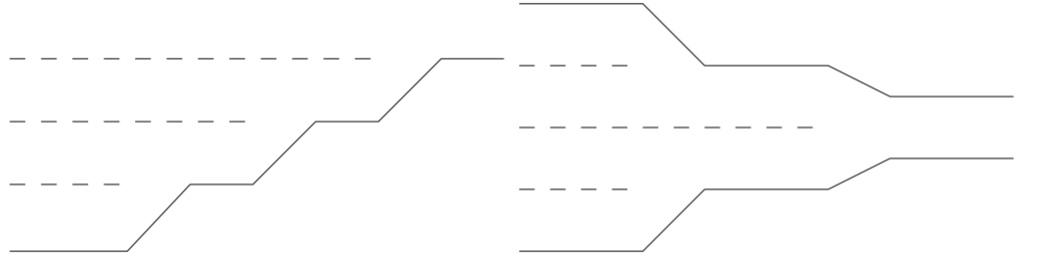
\includegraphics[width=12cm]{Two_Merging_Method.png}
\caption{Two Merging Methods} \label{fig:Two Merging Methods}
\end{figure}
\\
In the figure above, the number of traffic lanes decreases from 4 to 1. Although the number of traffic lanes cut down are the same in these two scenarios, the efficiency is different. In the second way, cars from two sides could begin "merging" at the same time, while cars in the first scenario could only merge from one lane to the neighbor lane one by one. Additionally, it is obvious that merging from one side costs more than merging from two sides. Therefore, in our model, the second method of merging is considered. 
\item
In the next section, we would assume that there's no self-driving(automated) car and all the tollbooths are of the same type. After the construction of the model, we will put the traffic situation, autonomous vehicles and different types of toll collection booths(human-staffed, exact-change and electronic tollbooths) into consideration to see how these factors affect our model.
\end{itemize}
\noindent
Under the above and basic assumptions, we can set out to construct our model (show our approach in detail).

%============ Question Analysis ========================
\section{Analysis of the Problem}
In this section, the problem will be divided into two parts and analysis will be done to help form the model.

\subsection{Gate Selection of Vehicles at Fan-out Area}
As mentioned before, all the tollbooths and vehicles are identical. We also assume that the queueing pattern at the tollbooths follows the first come first serve policy. Additionally, vehicles waiting in line are not allowed to renege, that is to leave or change the queue while waiting. So the motorist coming after is much more likely to choose the tollbooth with the shortest queue, that is with least vehicles waiting. Therefore, the vehicles tend to be distributed evenly at the plaza among all the tollbooths, and remain the pattern of even distribution while coming out of the tollbooths into the fan-in area since they all experience the same service time.

\subsection{Merging Pattern at Fan-in Area}
After toll, here comes a new stage: all vehicles set out at the speed of zero and merge at those merging points. Note that, since changes in flow occur smoothly and slowly, traffic flow(the number of vehicles in unit time) is usually considered to be roughly constant at any given moment. In other words, we could describe this process as a Poisson process where events happen continuously and independently at a constant average. Therefore, the traffic inter-arrival time must follow an exponential distribution before merging.[1]\\
\\
Given the roadway must narrow back from a number of tollbooth lanes to its normal width, common solutions used today are: 
\begin{itemize}
\item cut down the number of lanes from one side gradually
\item force a sharp merge at a relatively low speed
\end{itemize}
\noindent
Our solution to the problem will consider the fan-in shape which forces vehicles to merge from two side of the road to the middle, tending to minimize the waste time and construction cost.

%============= Construction of the model ===============
\section{Construction of the model}
\subsection{Queuing Theory}
Under our hypothesis, vehicles wait for the service of toll collection in tollbooths and may stop to waste time waiting for merging at the merging points. To model such process where customers line up to wait for service, we apply Queuing Theory.[2] It is common to use the symbols:
\begin{itemize}
\item $\lambda$ to be the mean or average number of arrivals per time period, i.e. the mean arrival rate.
\item $\mu$ to be the mean or average number of customers served per time period, i.e. the mean service rate.
\end{itemize}
We use notation system A/B/C to classify queuing model, where[2]
\begin{itemize}
\item A represents the probability distribution for the arrival process, which is also exponential distribution as we mentioned in the last section;
\item B represents the probability distribution for the service process, which is exponential distribution as we mentioned in the last section;
\item C represents the number of channels(servers), which is \# of tollbooths here.
\end{itemize}

\begin{table}[h]
\begin{center}
 \begin{tabular}{||c c c||} 
 \hline
 Characteristics & Symbols & Description \\ [0.5ex] 
 \hline\hline
 A & M & Exponential Distribution \\ 
 \hline
 B & M & Exponential Distribution \\
 \hline
 C & 1, 2 ... $\infty$ & Ideal Model \\
 \hline
 D & 1, 2 ... $\infty$ & Ideal Model \\
 \hline
 E & FCFS & First come fist serve \\ [1ex] 
 \hline
\end{tabular}
\caption{Queue System Parameters}
\label{table:1}
\end{center}
\end{table}

\noindent
In our model, it is M/M/C queuing system where M represents for a Poisson arrival distribution(exponential inter-arrival distribution) and C represents there are C tollbooths. By Burke's Theorem[3], the outcoming stream from the toll plaza also has the exponential distribution with the same rate as the arrival stream. This property will be used in the queue model of merging points.

\subsection{Merging Points and Process}
In the model, the number of traffic lanes decreases one after each merging point and all merging points are two-to-one merging points. For simplification, we assume that at the merging point, the vehicle on the main lane will drive first and the vehicle on the other lane will stop to wait if it cannot merge at that moment.

\subsection{Probability and Arrival Rate}
Consider the situation with L lanes and B tollbooths, where \(B, L \in \mathbb{N}\) and \(B\geqslant L\). We merge from both side by one lane simultaneously, so the total number of merging points at one side is \(\frac{B-L}{2}\) if \(B \equiv L \mod 2\), \(\frac{B-L-1}{2}\) on one side, \(\frac{B-L+1}{2}\) on the other side when \(B \equiv L+1 \mod 2\). However, at every merging point, arrival rate equals to the traffic flow it receives, so they are different among merging points.\\
\begin{figure}[h]
\small
\centering
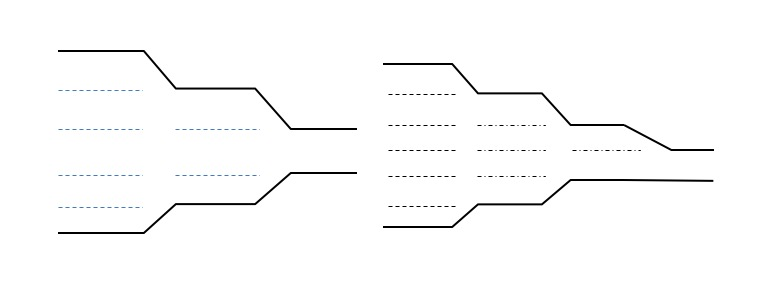
\includegraphics[width=12cm]{562831237.jpg}
\caption{Merging Model of Different B} \label{fig: Merging Model of Different B}
\end{figure}
\\
When  \(B \equiv L \mod 2\), the two sides are symmetric, so we may only consider one side.\\
\\
At the first merge point, the arrival rate is\\
\[
\lambda = \frac{2}{B} \times \phi
\]
since it bears the vehicles from the left-most two lanes.\\
\\
\noindent
At the second merge point, the arrival rate is\\
\[
\lambda = \frac{3}{B} \times \phi
\]
since it bears the vehicles from the left-most three lanes.\\
\\
So we may say that at the \(\frac{B-L}{2}\)-th merging point, the arrival rate is\\
\[
\lambda = \frac{B-L+1}{B} \times \phi
\]
When \(B \equiv L+1\mod 2\), the two sides are not symmetric. We may first consider merge from B tollbooths to (L+1) lanes. Then the method is the same as when \(B \equiv L \mod 2\), substituting L with (L+1). So at the \(\frac{B-L-1}{2}\)-th merging point, the arrival rate is\\
\[
\lambda = \frac{B-(L+1)+1}{B} \times \phi
\]
\\
There is still one merge point that will merge the (L+1) lanes to L lanes. So at this point, the arrival rate is\\ 
\[
\lambda = \frac{B-(L+1)+1}{B} \times \phi \times \frac{B+1}{B}
\]

\section{Calculating and Simplifying the Model}
\subsection{Appearing Variables}
\begin{itemize}
\item Total Traffic Flow($\phi$). According to the Institute of Transportation Engineers[4], the maximum traffic flow of one lane is 2000/hour. Light and heavy traffic condition have different value of $\phi$. In New Jersey, the number of vehicles per lane per hour is 1300[5].
\item Service Rate at the Merging Point:
\begin{itemize}
\item No other cars: $\mu_{a}$. Since after getting into the highway, vehicles should speed up to at least 40 km/h. By average car parameters, we estimate the acceleration as $2m/s^2$. The duration is approximately 1.67 seconds.\\
\[
\mu_{a} = \frac{3600}{1.67 s} = 2160/hr
\]
\item Merging Needed: $\mu_{b}$. To estimate the service rate when merging needed, we use the similar approach. Assume the merging occurs safely and efficiently, then the distance between two vehicles tends to be the safety distance, which is the length of the vehicle(speed is low in this scenario). From NJTA, 96\% of vehicles are cars and 4\% are trunks and buses, so we estimate the size of the car as 4.5 meters[5]. Therefore the average service time is approximately 3 seconds.\\
\[
\mu_{b} = \frac{3600}{3 s} = 1200/hr
\]
\end{itemize}
\end{itemize}

\subsection{Wasting Time(W)}
\subsection{Construction Cost(C)}

%============== Result of the model =====================
\section{The Model Results}

%========== 模型的实效分析(适应性说明)======================
\section{Validating the Model} 

\section{Conclusions}

%============ 总体评价 ====================================
\section{Evaluation: Strengths and weaknesses}
Like any model,the one present above has its strengths and
weaknesses. Some of the major points are presented below.

\subsection{Strengths}
\begin{itemize}
\item \textbf{Applies widely}
\end{itemize}

\subsection{Weakness}

\begin{thebibliography}{99}
\raggedright
\bibitem{1} Modeling Toll Plaza Behavior Using Queuing Theory. 2005. Retrieved from http://www.math.washington.edu/~morrow/mcm/cary05.pdf
\bibitem{2} Queuing Theory. J. E. Beasley. Retrieved from http://people.brunel.ac.uk/~mastjjb/jeb/or/queue.html
\bibitem{3} Burke's Theorem and Networks of Queues. M.I.T. Retrieved from https://ocw.mit.edu/courses/electrical-engineering-and-computer-science/6-263j-data-communication-networks-fall-2002/lecture-notes/Lecture7.pdf
\bibitem{4} Institute of Transportation Engineers, Traffic Engineering Handbook, Ed. James L. Pline, Prentice Hall, Englewood Cliffs, NJ, 1992.
\bibitem{5} Road User Cost Manual. New Jersey Turnpike Authority. Retrieved from http://www.state.nj.us/turnpike/documents/NJTA\%20Road\%20User\%20Cost\%20Manual.pdf
\end{thebibliography}